\subsubsection {Analisi al variare di P}
Anche al variare della probabilità di perdità si osserva (figura \ref{p}) un andamento 
abbastanza lineare fino a valori vicini al 60\%, da questo punto in
poi però, si ha una rapida divergenza e le prestazioni peggiorano
drasticamente.\\
Confermate, anche in questo caso, le peggiori prestazioni della versione
con timeout adattativo rispetto a timeout fisso per probabilità di perdita
elevate.
\begin{figure}[!ht]
	\centering
	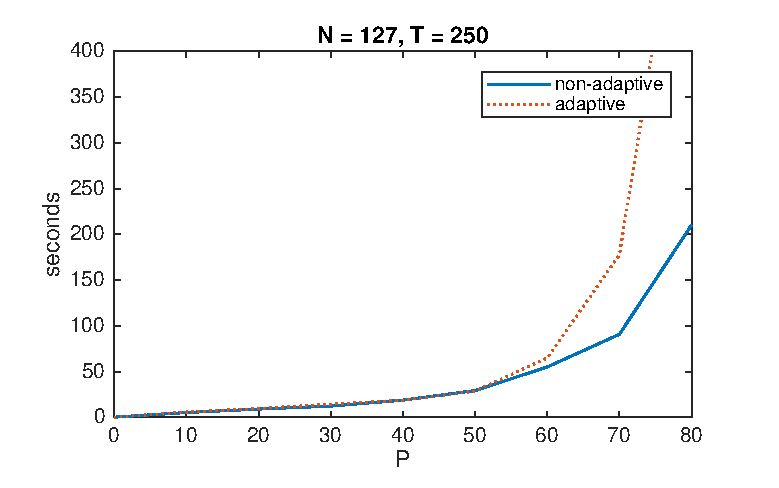
\includegraphics[scale=0.8]{images/P_N127_T250}
	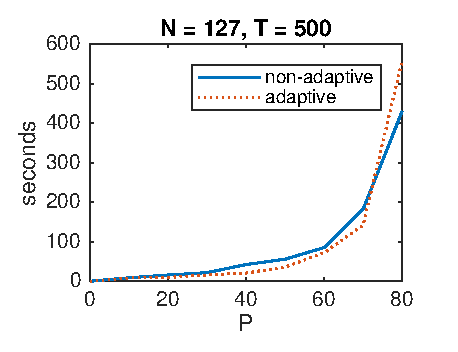
\includegraphics[scale=0.8]{images/P_N127_T500}
	\caption{prestazioni al variare della probabilità di perdita P,
			 ampiezza finestra N = 127, timeout minimo T = 250 ms e 
			 timeout normale T = 500 ms}
	\label{p}
\end{figure}
\newpage
